\documentclass[a4paper,11pt]{article}
\usepackage{a4wide}
\usepackage{fullpage}
\usepackage[utf8x]{inputenc}
\usepackage[slovene]{babel}
\selectlanguage{slovene}
\usepackage[toc,page]{appendix}
\usepackage[pdftex]{graphicx} % za slike
\usepackage{setspace}
\usepackage{color}
\usepackage[table]{xcolor}
\usepackage{tabularx}
\usepackage{float}
\usepackage{hhline}
\definecolor{light-gray}{gray}{0.95}
\usepackage{listings} % za vključevanje kode
\usepackage{hyperref}
\renewcommand{\baselinestretch}{1.2} % za boljšo berljivost večji razmak
\renewcommand{\arraystretch}{1.2}
\hyphenpenalty=10000
\newcolumntype{Y}{>{\centering\arraybackslash}X}

\title{Temperaturna plošča: serijski algoritem}
\author{Rok Grmek, Matej Klemen}
\date{\today}

\begin{document}

\maketitle

\section{Opis problema (in motivacija?)}


\section{Opis uporabljene metode}
\subsection{Algoritem}

\subsection{Uporabljene knjižnice}

\section{Rezultati}

\indent \par Program je bil testiran na sistemu, katerega specifikacije so navedene v tabeli \ref{tabela-specifikacije}.

Pri testiranju sva se omejila na fiksno velikost temperaturne plošče ($500 \times 500$) in spreminjala zgolj število iteracij. Za vsako izbrano število iteracij sva program 100-krat zagnala in vsakič izmerila čas izvajanja. Iz meritev sva nato izračunala povprečni čas izvajanja in standardno napako meritve, ki predstavlja razpršenost meritev okoli povprečnega časa izvajanja. Rezultati so navedeni tabelarično v tabeli \ref{tabela-rezultati-sekvencni} in na grafu, ki je prikazan na sliki \ref{graf-rezultati-sekvencni}.
\begin{table}[H]
\begin{center}
\caption{Specifikacije testnega sistema.}
\label{tabela-specifikacije}
\begin{tabularx}{\textwidth}{|YY|}
\hhline{==}
\rowcolor{light-gray} Procesor & Intel Core i5-4210U\tabularnewline
Frekvenca procesorja & 1.70GHz \tabularnewline
\rowcolor{light-gray} Število jeder & 2 \tabularnewline
Maksimalno število niti & 4 \tabularnewline
\rowcolor{light-gray} Velikost predpomnilnika & 3MB \tabularnewline
Pomnilnik & 16GB DDR3 \tabularnewline
\rowcolor{light-gray} Grafična kartica & NVIDIA GeForce 820M 2GB DDR3 \tabularnewline
\hhline{==}
\end{tabularx}
\end{center}
\end{table}

\begin{table}[H]
\caption{Povprečni čas izvajanja in standardna napaka meritev v odvisnosti od števila iteracij.}
\label{tabela-rezultati-sekvencni}
\begin{center}
\begin{tabularx}{\textwidth}{YYY}
\hhline{===}
Število iteracij & Povprečni čas izvajanja [s] & Standardna napaka [s] \tabularnewline
\hhline{===}
500 & 1,698 & 0,001 \tabularnewline
1000 & 3,400 & 0,003 \tabularnewline
2000 & 6,780 & 0,003 \tabularnewline
5000 & 17,757 & 0,103 \tabularnewline
10000 & 33,972 & 0,026 \tabularnewline
20000 & 67,940 & 0,024 \tabularnewline
\end{tabularx}
\end{center}
\end{table}

\begin{figure}[H]
\begin{center}
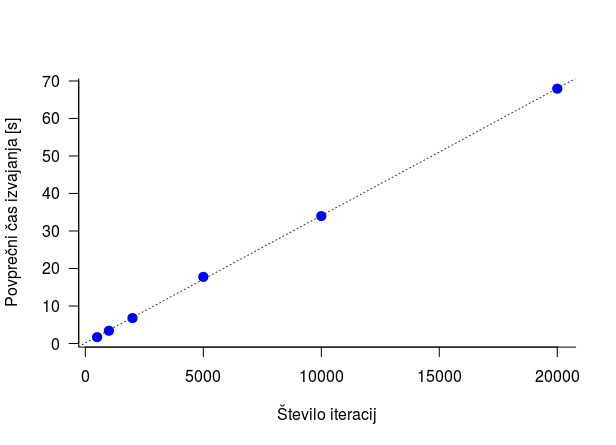
\includegraphics[scale=0.8]{rezultati_porocilo1.png}
\end{center}
\caption{Graf, ki prikazuje povprečni čas izvajanja programa v odvisnosti od števila iteracij.}
\label{graf-rezultati-sekvencni}
\end{figure}

\section{Literatura? (verjetno ne)}
\end{document}